\documentclass[10pt, reqno]{article}
\usepackage[left=3cm,right=3cm,top=3cm,bottom=3cm]{geometry}
\geometry{letterpaper}                   
\usepackage[utf8]{inputenc}
\usepackage[numbers]{natbib}
\usepackage{graphicx}
\usepackage{color}
\usepackage{amssymb}
\usepackage{verbatim}
\usepackage{amsmath}
\usepackage{epstopdf}
\usepackage{enumerate}
\usepackage[format=plain,font=footnotesize,labelsep=newline,singlelinecheck=false,justification=justified,margin=1cm]{caption}
\DeclareGraphicsRule{.tif}{png}{.png}{`convert #1 `dirname #1`/`basename #1 .tif`.png}
\setlength{\parindent}{25pt}
\renewcommand{\abstractname}{}

\title{Python calculations of Bohmian trajectories}
\author{Dane Odekirk} 
\date{December 12th, 2012}                                         


\begin{document} 
\maketitle 
\pagebreak

\begin{abstract}
  \noindent 
  {\bf Abstract. } 

  %[TODO: SEPARATE SYSTEMS IS NOT CORRECT SINCE ITS BOTH 2 INTERFEREING WAVE PACKETS. RELATED SYSTEMS IS BETTER]
  The Python programming language is used to calculate Bohmian trajectories for two interfering wave-packets. 
  A fourth-order Runge-Kutta is implemented to numerically solve the differential equations that describe the trajectories.
  Trajectories are computed on a 1.7Ghz Core i5 processor using Python version 2.7.2 with the NumPy, SymPy and Matplotlib packages.
  All results agree with current de Broglie-Bohm theory.
  The Python scripts are referenced in the appendix.

\end{abstract}




\section{Introduction}

  Quantum mechanics is famed for introducing uncertainty to a once certain world.
  The de Broglie-Bohm theory rectifies this with a causal interpretation of quantum mechanics by 
    prescribing definite trajectories to particles without sacrificing predictive accuracy.
  This is a stark contrast to the Copenhagen interpretation where a system's behavior is nondeterministic.  
  The ramifications of the de Broglie-Bohm interpretation remedy the concept of wave-particle duality since
    quantum systems can be predicted without losing the particles.
  This gives rise to a narrative of the particles that can be discussed, analyzed and is not hidden nor ignored as it with 
    the Copenhagen interpretation.

  The de Broglie-Bohm theory proposes that a system of $n$ particles has trajectories described by 

  \begin{equation} \label{eq:trajectories}
    \dot{r} = \frac{\hbar}{m_i}\text{Im}[\frac{ \nabla_{i} \Psi(r_1,\dots,r_n,t)}{\Psi(r_1, \dots, r_n, t) } ]
  \end{equation}

  \noindent
  for each particle $i$; where $\Psi$ is the total wave function \cite{guay}.
  This is recognized as the guiding equation.
  First presented by de Broglie in 1927, the de Broglie interpretation of quantum mechanics was quickly abandoned after a confident rebuttal by Pauli during a conference.
  Although de Broglie's defense was accurate, Pauli and his objections garnered support and momentum away from the de Broglie interpretation
    and it was eventually abandoned as the Copenhagen interpretation became more popular.
  In 1952, however, Bohm reintroduced the theory with proper rebuttals of Pauli's objections \cite{bohm}.

  Bohm's theory, also known as Bohmian mechanics or de Broglie-Bohm theory, is formulated via the Schrödinger equation \cite{bohm}.
  To illustrate, consider the one-particle Schrödinger equation given by 
    \begin{equation}
      i \hbar \frac{\partial}{\partial t} \Psi(\mathbf{r},t) = \Bigg[ \frac{-\hbar}{2m} \nabla^2 + V(\mathbf{r},t) \Bigg] \Psi(\mathbf{r},t)
    \end{equation}
  where $V$ is the potential and $\Psi$ is the wave function.
  When the wave function is written in Euler form 
    \begin{equation}
      \Psi(\mathbf{r},t) = \sqrt{P} \exp(\frac{iS}{\hbar}) 
    \end{equation}
  where $P$ and $S$ are real, dimensionless functions, the Schrödinger equation can be evaluated.
  Separating the result into real and imaginary parts yields the following equations:
  \begin{align} 
    \frac{\partial P}{\partial t} &= - \mathbf{\nabla} \cdot (P \frac{\mathbf{\nabla} S}{m}) \label{eq:bohm1} \\
    %\frac{\partial S}{\partial t} &= - \frac{1}{2}( \mathbf{\nabla}S^2 - Q - V(\mathbf{r}) \label{eq:bohm2} )
    \frac{\partial S}{\partial t} &= - \frac{1}{2} \Bigg[ \frac{(\nabla S)^2}{m} - 2V(\mathbf{r}) + Q \label{eq:bohm2} \Bigg] 
  \end{align}
  where Q is given by
  \begin{equation} \label{eq:quantumpotential}
    Q = -\frac{\hbar^2}{2m}\frac{\nabla^2 \sqrt{P}}{\sqrt{P}}
  \end{equation}
  For the remainder of this paper, the constants $m$ and $\hbar$ are set equal to one.
    
  Bohm recognized when evaluating equation (\ref{eq:bohm1}) at the classical limit, $ \hbar \rightarrow 0 $, 
    that $S$ is the solution to the classical Hamilton-Jacobi equations of motion \cite{bohm}.
  The Hamilton-Jacobi equations are accurate for classical systems, however,
    are incomplete for the quantum realm.
  Specifically, the function $Q$ approaches zero classically and only exists at the quantum limit.
  This function $Q$ is known as the quantum potential and is the difference between the quantum and classical Hamilton-Jacobi equations of motion.
  It also plays a significant role in the behavior of de Broglie-Bohm particle trajectories.
  Bohm quotes the following theorem \cite{bohm} 
  \begin{quotation}
    \noindent
    If we consider an ensemble of particle trajectories which are solutions of the equations of motion,
    then it is a well-known theorem of mechanics that if all these trajectories are normal to any given surface of constant $S$,
    then they are normal to all surfaces of constant $S$, 
    and $\nabla S(x) / m $ will be equal to the velocity vector, $\mathbf{v}(\mathbf{x})$,
    for any particle passing the point $ \mathbf{x} $.
  \end{quotation}
  Applying this theorem yields two results.
  First, equation (\ref{eq:bohm1}) can be rewritten in terms of a particle's velocity since $\nabla S(x)$ is equal to the velocity $\mathbf{v}$.
  P is therefore consistent with the probability density for these particles,
    where $P\mathbf{v}$ represents the mean current of particles.
  Equation (\ref{eq:bohm1}) then represents the conservation of probability.
  Second, equation (\ref{eq:bohm2}) is consistent with the Hamilton-Jacobi for a system of such particles.
  Unlike its classical counterpart, however, the particles are affected by two types of potentials: 
    the classical potential $V$ and the quantum potential $Q$.

  To summarize, solving the Schrödinger equation with a wave function in Euler form results in a set of equations.
  These set of equations are equal to the Hamilton-Jacobi equations of motion at the classical limit 
    and introduce the new quantum potential $Q$ at the quantum limit.
  Furthermore, they imply a set of calculable trajectories for each particle in the system;
    defining a narrative that is nonexistent in the Copenhagen interpretation.

  In order to calculate Bohmian trajectories of a particle, its $x$ and $y$ position must be determined at any given time $t$.
  The $x$ component of the particle's position can be found via 
  \begin{equation}
    x(t) = x(0) + k_x t 
  \end{equation}
  where $k_x$ is the velocity in the $x$ direction \cite{guay}.
  This simplifies the calculation by allowing us to focus specifically on the $y$ coordinate realizing that 
    the $x$ coordinate is simply proportional to the time $t$.
  The $y$ coordinate of a particle at time $t$ is found by feeding the wave function $\Psi$ that describes the system into equation (\ref{eq:trajectories}).
  With initial random values of $t_0$ and $y_0$, equation (\ref{eq:trajectories}) is evaluated over iterations of times $t$ between $t_i$ and $t_f$ to calculate the 
    particle's $y$ coordinate at each specific time $t$.
  Compiling this solution with the $x$ coordinate yields the trajectory of a particle with initial position $x_0$ and $y_0$.
  
  In this paper a fourth-order Runge-Kutta is implemented to compute the Bohmian trajectories defined by equation (\ref{eq:trajectories}) \cite{dowsa}.
  Interfering wave packets are investigated for two related systems.
  Python 2.7.2 is the programming language of choice because of its syntax, built in debugger, and open-sourced scientific packages.
  The language itself is freely available and open-sourced as well.
  The specific packages used are NumPy, SymPy and Matplotlib which provide numerical functions, symbolic math and plotting functions respectively.
  Full understanding of these packages is not necessary to understand or run the Python code; 
    although some background knowledge of their capabilities, purposes and implementations could prove helpful.



\section{Double-slit experiment}

  Bohmian trajectories are calculated for a double-slit setup.
  The classical double slit experiment consists of the following parts:
    a source that emits particles,
    a barrier with two slits A and B cut into it,
    and a screen that captures and records the particles.
  This is illustrated in Figure \ref{fig:double-slit}.
  The system implemented in this investigation shares these characteristics and makes no special alterations to the traditional experimental setup.

  \begin{figure}[!ht]
    \centerline{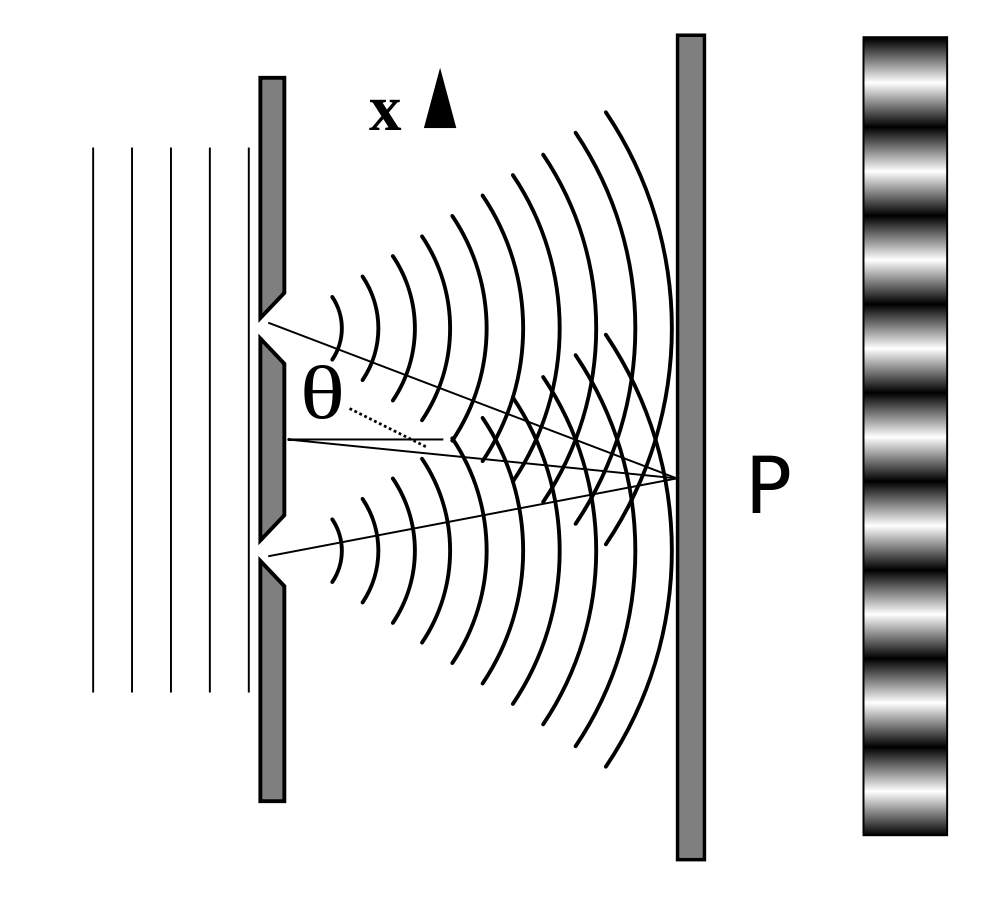
\includegraphics[scale=.2]{./imgs/double-slit.png}}
    \caption{
      Traditional double slit setup \cite{wiki}. 
      Bohmian trajectories are calculated for such a system.
    }
    \label{fig:double-slit}
  \end{figure}

  When a particle goes through either slit its wave function is described by $\psi_A(\mathbf{r},t)$ and $\psi_B(\mathbf{r},t)$ for slits A and B respectively.
  The wave that leaves the slit has an exact solution described by the following time-dependent equation \cite{guay-double-slit}
  \begin{equation}
    \label{eq:partial}
    \psi_n(\mathbf{r},t) = (2\pi\sigma^2)^{-1/4} \exp \Bigg[ \frac{(y_i - Y)^2}{4 \sigma_{0} \sigma_{t}} + i \Bigg[ k_x x_i - \frac{k_x^2 t}{2} \Bigg]\Bigg]
  \end{equation}
  where 
  \begin{equation}
    \sigma_{t} = \sigma_{0}(1 + \frac{it}{2\sigma^2_0})
  \end{equation}
  This definition assumes the particles are traveling in free space and the classical voltage $V$ is zero.
  The total wave function needed to calculate trajectories with equation (\ref{eq:trajectories}) is described by the following equation
  \begin{equation}
    \label{eq:total-wave-function}
    \Psi(\mathbf{r},t) = N [\psi_A + \psi_B ]
  \end{equation}
  where $\psi_A$ and $\psi_B$ are defined by equation (\ref{eq:partial}) and $N$ is a normalization constant.

  Figures \ref{fig:2d0} and \ref{fig:2d1} illustrate the time-dependence of the wave function $\Psi$.
  Both the real and imaginary parts of of the wave function, described by equation (\ref{eq:total-wave-function}), are plotted at times $t=0$ and $t=1$. 
  Both Figures \ref{fig:2d0} and \ref{fig:2d1}, span $y$ values from -13 to 13 with a spacing of 0.01, accounting for 2600 points to be plotted.
  Good consistency is found between these figures and figures in reference \cite{guay-double-slit} on which these graphs are based.
  The code to produce these figures is shown in appendix \ref{appendix:real-imag}.

    \begin{figure}[!ht]
      \centerline{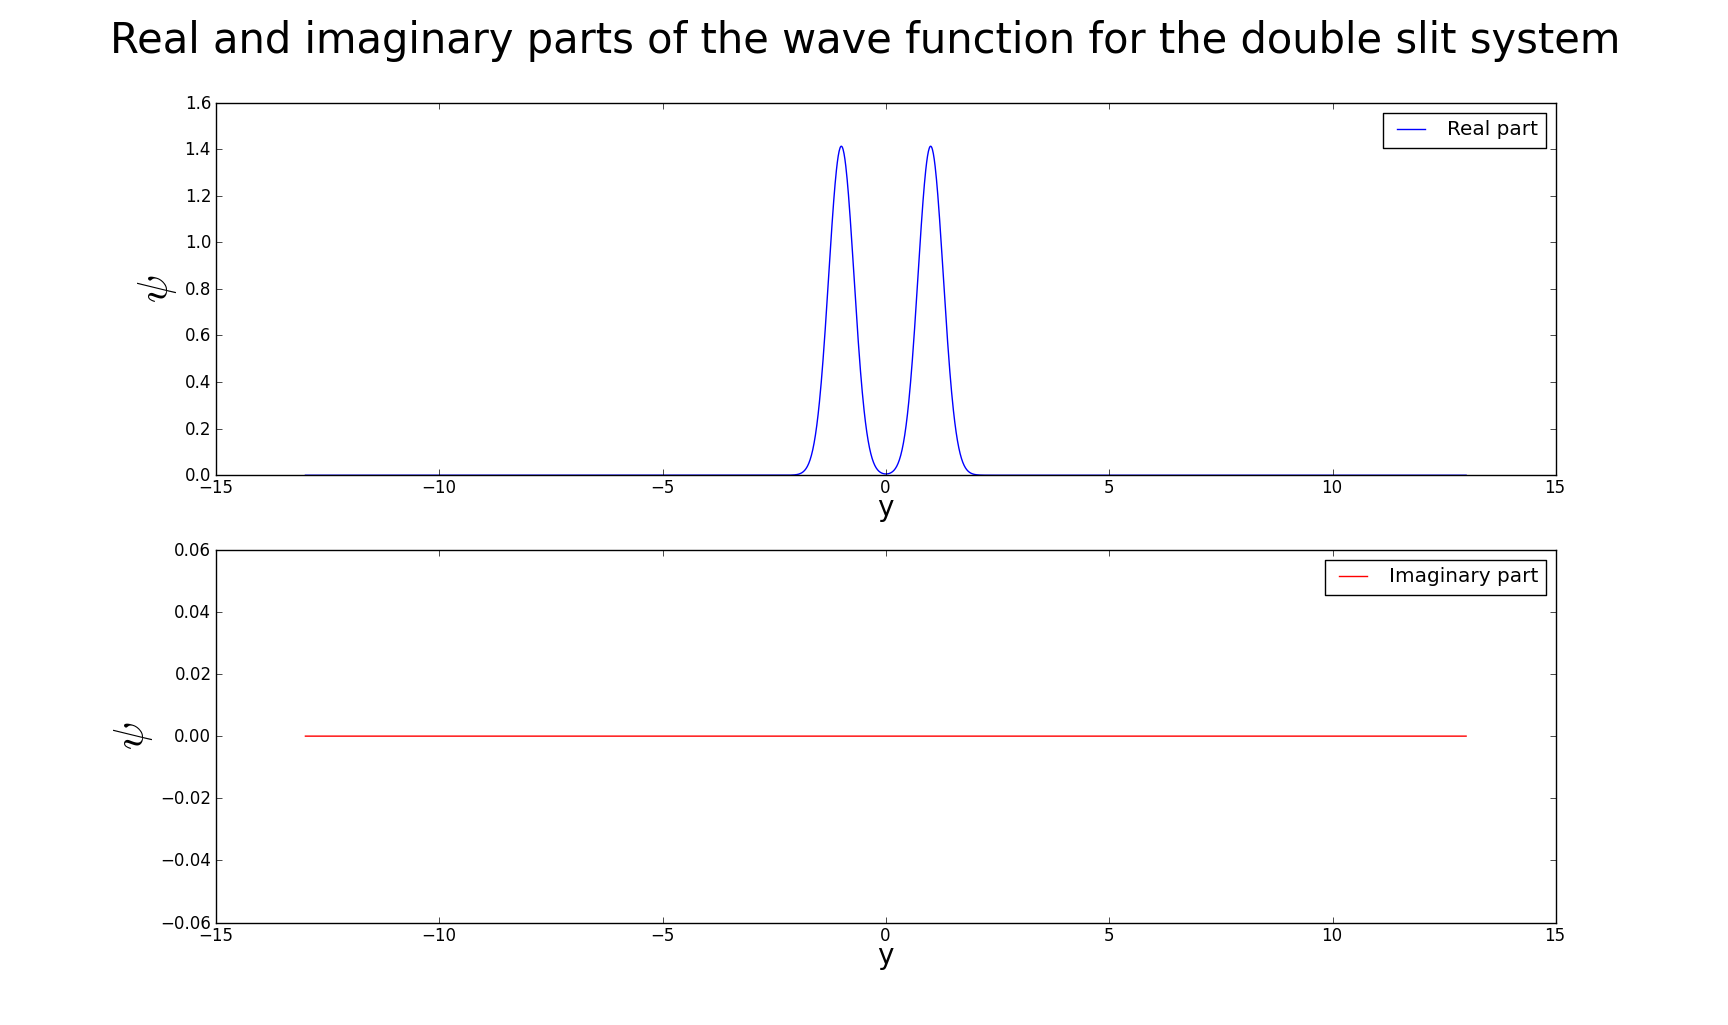
\includegraphics[scale=.3]{./imgs/double-slit-real-imaginary-parts-t0.png}}
      \caption{
        Two-dimensional breakdown of the real (blue) and imaginary (red) parts of equation (\ref{eq:total-wave-function}) evaluated at $t=0$.
        Values of $y$ span from -13 to 13 with spacing $\Delta y$ of 0.01.
      }
      \label{fig:2d0}
    \end{figure}
    \begin{figure}[!ht]
      \centerline{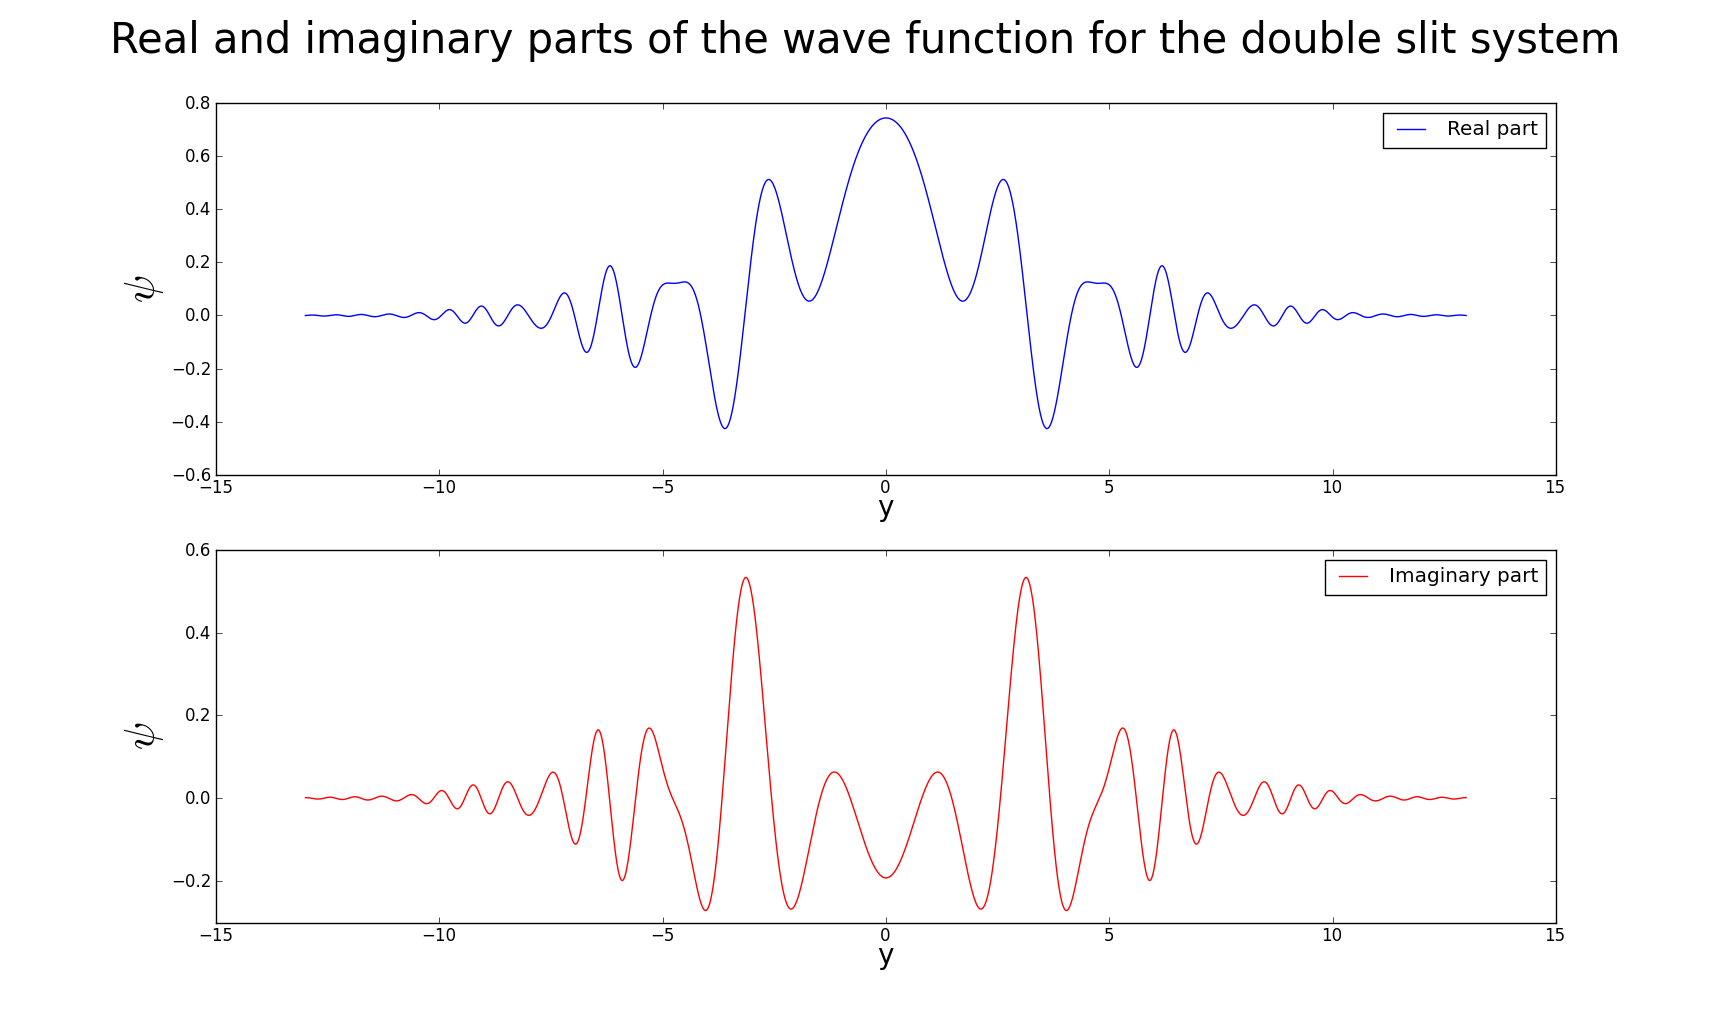
\includegraphics[scale=.3]{./imgs/double-slit-real-imaginary-parts-t1.png}}
      \caption{
        Two-dimensional breakdown of the real (blue) and imaginary (red) parts of equation (\ref{eq:total-wave-function}) evaluated at $t=1$.
        Values of $y$ span from -13 to 13 with spacing $\Delta y$ of 0.01.
      }
      \label{fig:2d1}
    \end{figure}

  According to equation (\ref{eq:trajectories}) the imaginary part of the wave function plays an important role in guiding particles along their 
    Bohmian trajectories.
  For a more revealing perspective, the imaginary part of the wave function is plotted three-dimensionally over time in Figure \ref{fig:3d}
    with a color grading representing the gradient along its surface.
  Note that the $x$ axis has been replaced by the time $t$ as they are proportional to one another.
  Values for $y$ once again span between -13 and 13 with a spacing of 0.01 and
    values for $t$ span between 0 and 1 with a spacing of 0.01.
  These values are chosen on a rather subjective basis of time - as decreasing the spacing increases the computation time.
  Generating Figure \ref{fig:3d} takes approximately 1.35 seconds with the given values.
  The code to generate this graph is shown in appendix \ref{appendix:imaginary-surface}.

  Figure \ref{fig:3d} clarifies the underlying mechanisms that govern the Bohmian trajectories.
  Notice the imaginary parts of Figures \ref{fig:2d0} and \ref{fig:2d1} agree with the cross-section parallel to $x$ of Figure \ref{fig:3d} at times $t=0$ and $t=1$.
  The crest and troughs of the wave function govern the direction of the particle. 
  Higher crests require higher energy while the troughs require lower energy.
  The trajectories follow the path of lowest energy.
  Not depicted in Figure \ref{fig:3d} is the quantum potential $Q$ that also affects the trajectories - it is plotted in reference \cite{bohm}. 
  When $Q$ is plotted three-dimensionally, it also illustrates the crests and troughs that govern the particle's trajectory \cite{bohm}.

  Of more interest, however, is the concept of the trajectory. 
  The narrative behind the Copenhagen interpretation is one that focuses on predictions and observations while ignoring how the observation came to be.
  With the de Broglie-Bohm interpretation, the prediction is still valid however the particle's trajectory, or the history of how it arrived at the observation, 
    can still be calculated and discussed.
  For example, the de Broglie-Bohm interpretation shows that a particle does in fact go through a specific slit; either one or the other.
  It does not have a predictive measure to calculate which slit the particle will go through prior to reaching the slits, however, does define 
    a historical trajectory that leads to a single, specific slit.
  This is not the case in the Copenhagen interpretation where 
    the particle's probability wave passes through both slits and the concept of a physical particle passing through a single slit is irrelevant.


    \begin{figure}[!ht]
      \centerline{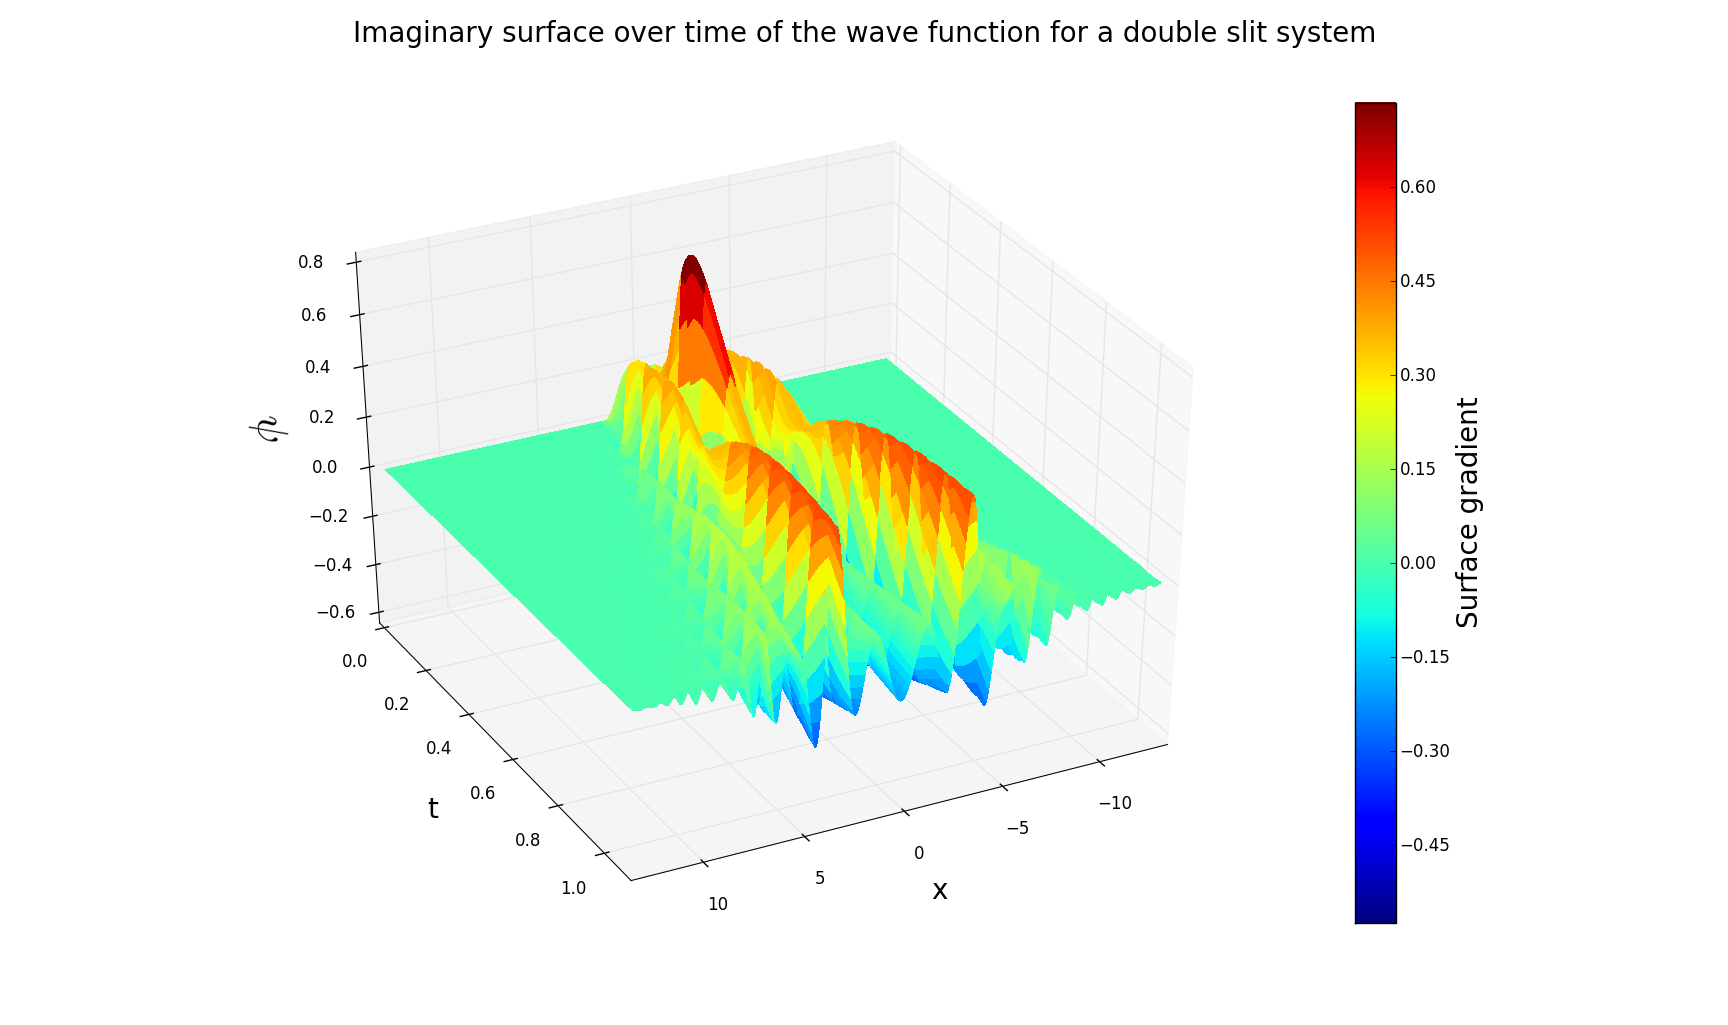
\includegraphics[scale=.4]{./imgs/double-slit-real-imaginary-parts-3d.png}}
      \caption{
        Three-dimensional plot of the imaginary surface of equation (\ref{eq:total-wave-function}) as it propagates through time.
        This figure exposes the physical importance of the wave function, which inevitably governs the path of particles at they traverse from $t=0$
      to $t=1$.
      }
      \label{fig:3d}
    \end{figure}

\section{Double-slit trajectories}

  Figures \ref{fig:trajsym}, \ref{fig:trajnonsym} and \ref{fig:trajnorm} plot the Bohmian trajectories for particles in a double slit setup; 
    numerically solved via Python.
  There are two main commonalities between these three figures.
  First, an interference pattern emerges in all three as expected. 
  This is promising since the double slit experiment does produce physical interference patterns that cannot be contradicted by the calculation.
  Second, all three figures exhibit trajectories that do not cross paths, which is an intrinsic characteristic of Bohmian trajectories.

  All the trajectories plotted in Figures \ref{fig:trajsym}, \ref{fig:trajnonsym} and \ref{fig:trajnorm} were calculated with the following constants:
    a distance between slits of 2 units, a slit width of 1 unit and an initial $x$ velocity of 0.1 units per second.
  The time spacing $\Delta t$ between calculated points is 1/100 seconds.
  Calculating the graphs takes approximately 26.4, 28.3 and 66.3 seconds respectively.
  The initial distribution is a random uniform distribution across each slits.
  The Python class that generates these plots is shown in appendix \ref{appendix:bohmian-trajectories}.

  \begin{figure}[!ht]
    \centerline{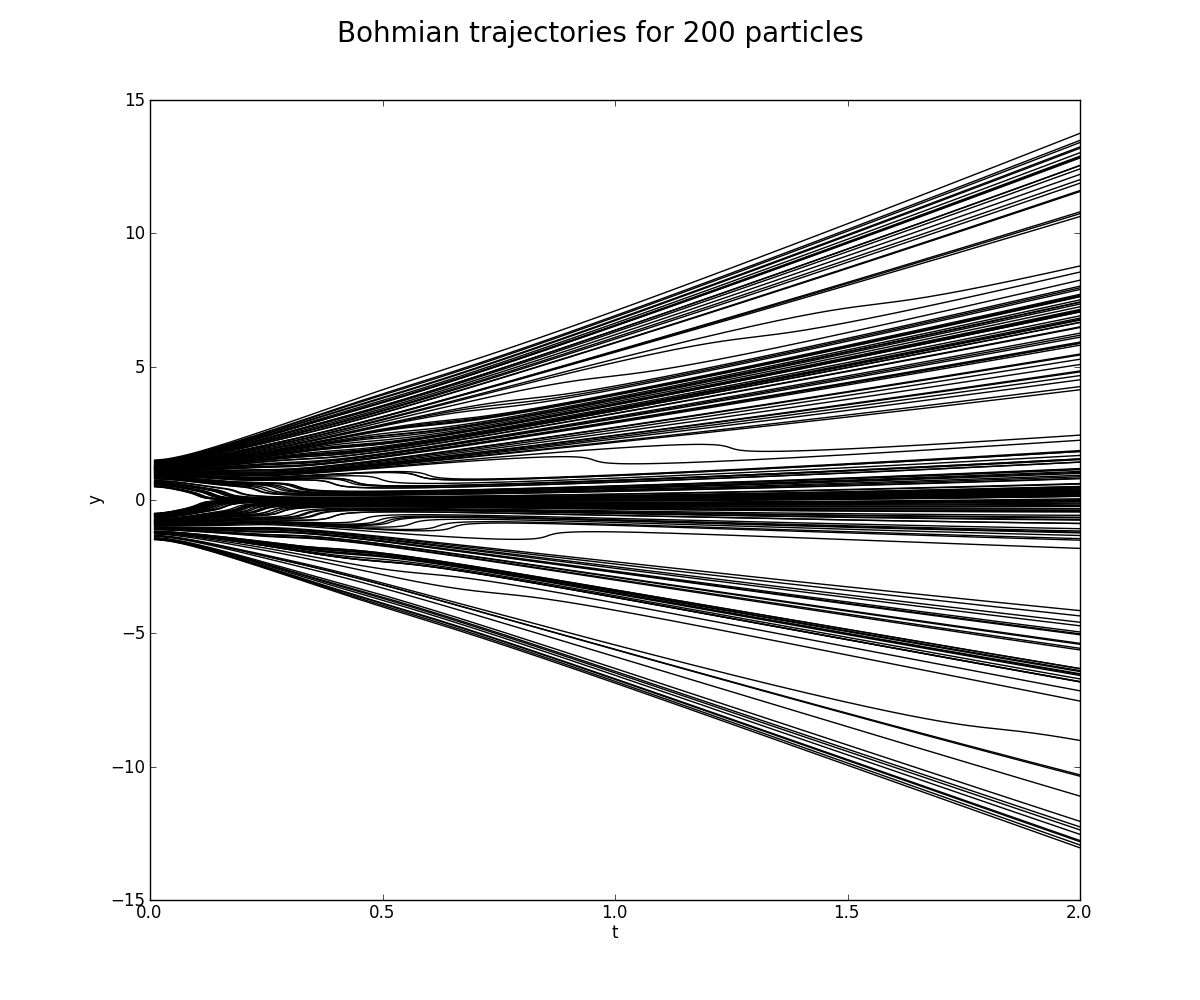
\includegraphics[scale=.3]{./imgs/200-bohmian-trajectories-85e4ecb6df758e2b.png}}
    \caption{
      200 particle trajectories with a random uniform distribution over each slit.
    }
    \label{fig:trajsym}
  \end{figure}

  \begin{figure}[!ht]
    \centerline{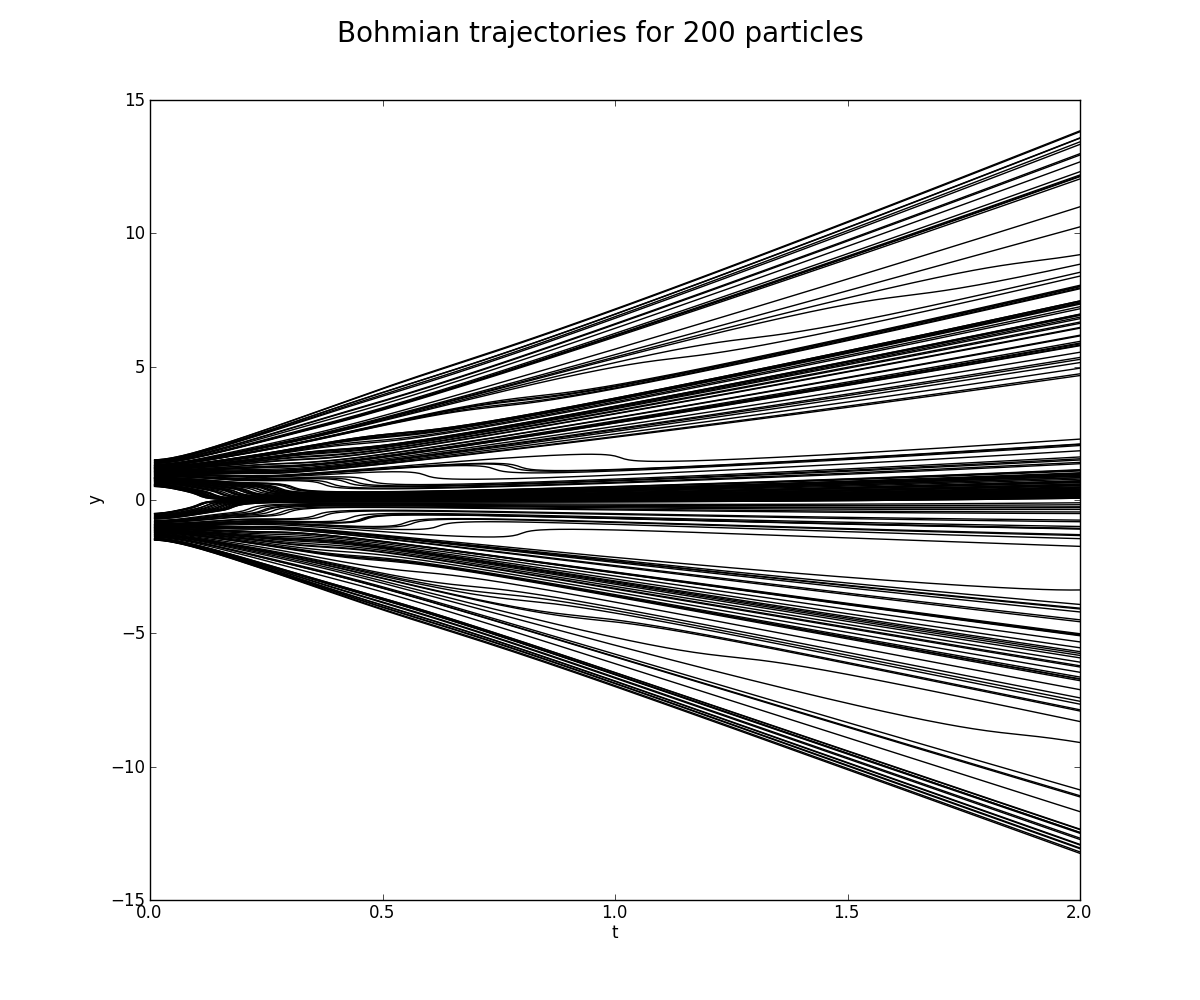
\includegraphics[scale=.3]{./imgs/200-bohmian-trajectories-3506320ca33960b0.png}}
    \caption{
      200 particle trajectories with an random uniform distribution over each slit. 
      There is no difference between this and Figure \ref{fig:trajsym} except the initial position of the particles.
    }
    \label{fig:trajnonsym}
  \end{figure}

  \begin{figure}[!ht]
    \centerline{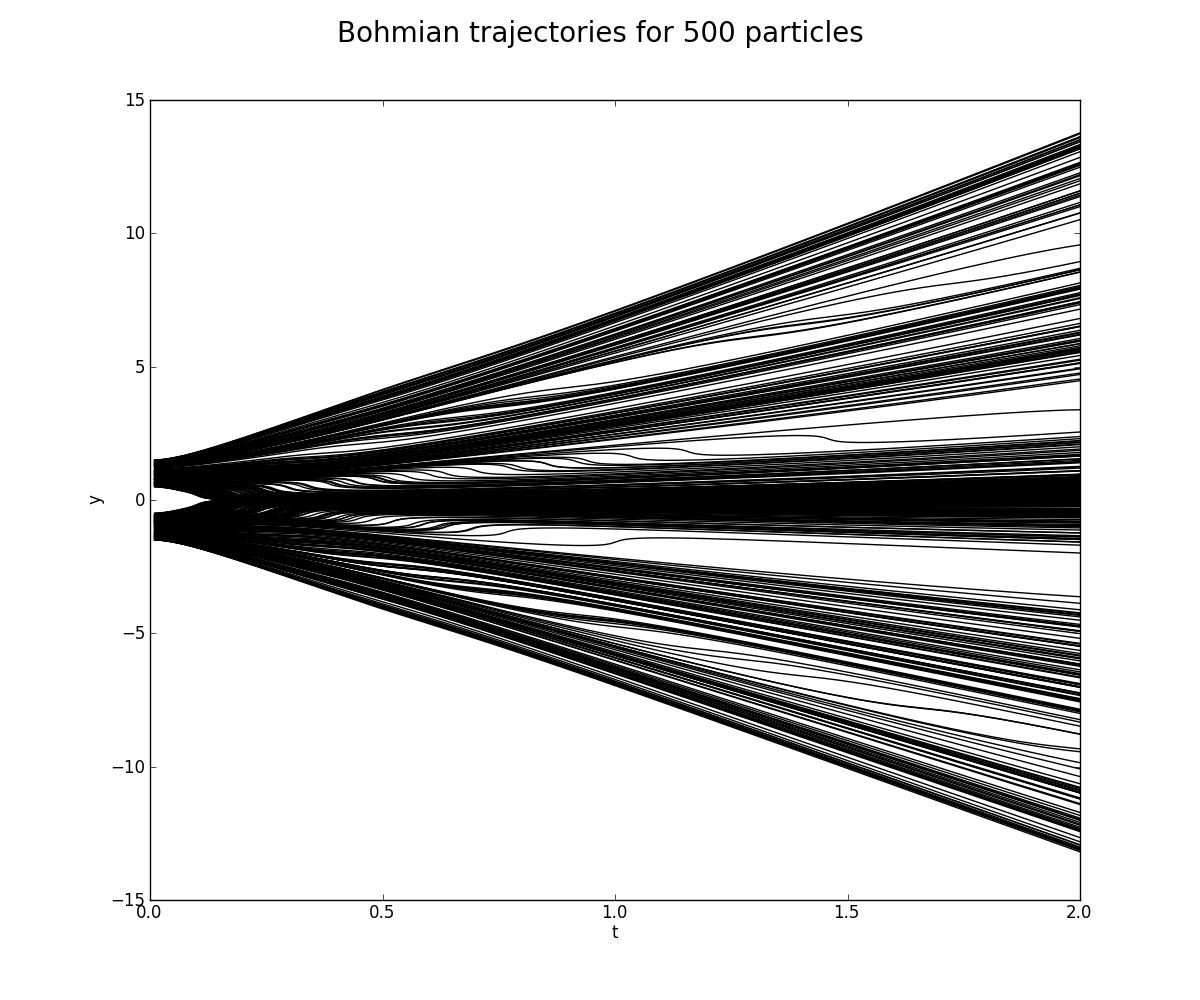
\includegraphics[scale=.5]{./imgs/500-bohmian-trajectories-693872239e5414e4.png}}
    \caption{
      500 particle trajectories with a random, uniform distribution over each slit.
    }
    \label{fig:trajnorm}
  \end{figure}
  \nocite{philippidis}

  The basic criteria for Bohmian trajectories appear correct.
  There is a visual departure from classical trajectories in Figures \ref{fig:trajsym}, \ref{fig:trajnonsym} and \ref{fig:trajnorm} as well.
  Classically, if a particle starts at the slit with a distinct position and velocity it will continue along the direction of the
    particle's velocity in a straight line unless acted upon by an external force.
  The trajectories depicted do not follow straight paths and appear to veer at specific points.
  The cause of these detours is the quantum potential given by equation (\ref{eq:quantumpotential}).
  It provides a force, in the quantum realm, that governs the particles into trajectories foreign to classical behavior.

  \begin{figure}
    \centerline{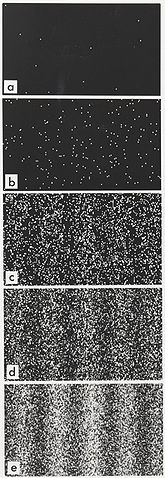
\includegraphics[scale=4.5]{./imgs/double-slit-results.jpg}}
    \caption{
    Screen results of the double slit experiment over time \cite{wiki}.
    }
    \label{fig:double-slit-results}
  \end{figure}

  When this experiment is performed, Figure \ref{fig:double-slit-results} illustrates what a screen registers at different times.
  Both the Copenhagen and de Broglie-Bohm interpretations predict this interference pattern.
  The Copenhagen interpretation, however, ignores an explanation of the particle itself until it is measured by the screen, 
    while the de Broglie-Bohm interpretation offers a narrative of the particle's trajectory.
  As stated previously, a fundamental distinction is the de Broglie-Bohm notion that a single particle goes through a specific slit.
  The probability wave used in the Copenhagen interpretation does not quite offer this distinction and
    suggests that the particle goes through both slits and interferes with itself.
  The trajectories in Figures \ref{fig:trajsym} and \ref{fig:trajnonsym} would be representative of a screen at time $c$ in Figure \ref{fig:double-slit-results}, 
    while Figure \ref{fig:trajnorm} would be representative of a screen at time $d$.

\section{Secondary setup and trajectories}

  The Python class used to generate the previous trajectories is extended to fit a new wave function.
  Similar to the double-slit experiment, this secondary setup consists of a source that emits particles and a screen that captures the particle.
  Instead of the particle going through two slits, however, it hits a beam-splitter with 50\% chance of the particle going
    in one direction or another.
  After passing through the beam-splitter the particle hits a mirror and reflects towards the screen as illustrated in Figure \ref{fig:interfering-setup}.

  \begin{figure}[!ht]
    \centerline{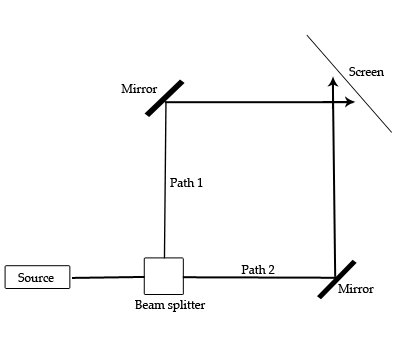
\includegraphics[scale=.6]{./imgs/secondary-setup.png}}
    \caption{
      The configuration setup for the interfering wave packet experiment.
    }
    \label{fig:interfering-setup}
  \end{figure}

  The wave packets are assumed to be Gaussian in nature and do not spread with time \cite{chaloupka}.
  Equation (\ref{eq:trajectories}) is used again to calculate the Bohmian trajectories for the wave function $\Psi$ that describes this system.
  The contour plot shown in Figure \ref{fig:interfering} illustrates the wave function $\Psi$ at times $t=-15$, $t=0$ and $t=15$ seconds 
    as the wave packets $\psi_A$ and $\psi_B$ propagate towards each other on intersecting paths.
  Initially, at $t=-15s$, the two wave packets are separate entities described by a single wave function traversing orthogonal paths.
  At $t=0$, the wave packets are completely superimposed upon each other forming an interference pattern with nodes and anti-nodes as the two Gaussian wave packets interfere.
  As the wave packets continue to propagate the interference pattern diminishes until eventually the wave packets are separate entities again;
    propagating along the same path as they initially were.
  The code to generate Figure \ref{fig:interfering} is shown in appendix \ref{appendix:contour-plot}.
  Code to generate a continuous animation of this contour plot is shown in appendix \ref{appendix:contour-plot-animated}.

  \begin{figure}[!ht]
    \centerline{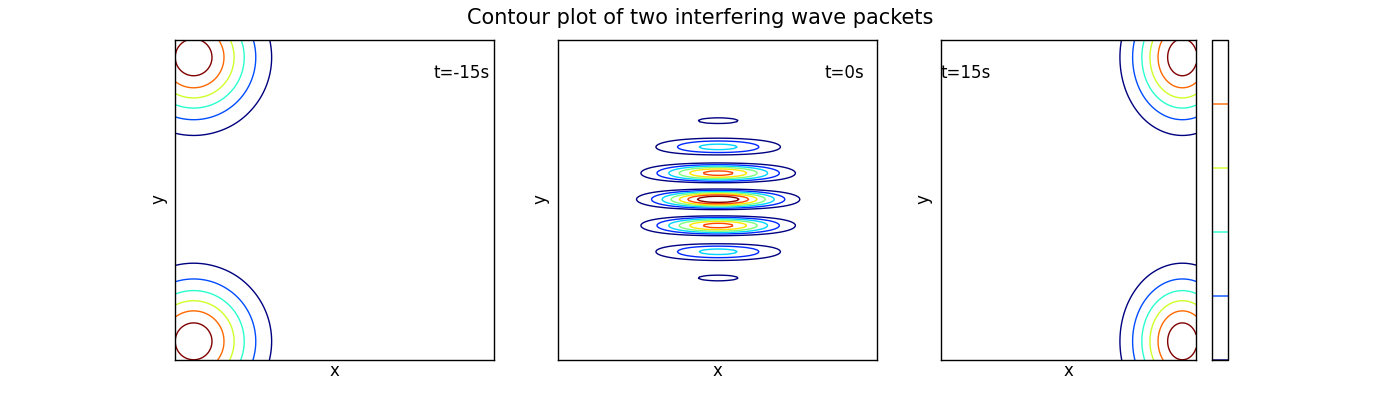
\includegraphics[scale=.5]{./imgs/contour-plot.png}}
    \caption{
      Contour drawing of two interfering wave packets at times $t=-15s$, $t=0s$ and $t=15s$.
    }
    \label{fig:interfering}
  \end{figure}

  Calculating the Bohmian trajectories for the system yields the trajectories plotted in Figure \ref{fig:interfering-trajectories}.
  The time $t$ spans from -15 seconds to 15 seconds with iterations of $1/100s$.
  The particles are initially distributed with equidistant spacing with the bottom and top packets offset by a 1/2 step to avoid symmetry over the $y=0$ axis.
  Plotting 100 trajectories takes approximately 5 minutes and 55 seconds.
  Again, the calculations only find the $y$ coordinate of each particle since the $x$ coordinate is proportional to the time $t$. 
  The Python code to generate Figure \ref{fig:interfering-trajectories} is shown in appendix \ref{appendix:secondary-trajectories} and is a 
    subclass of the Python class in appendix \ref{appendix:bohmian-trajectories} that accommodates the new initial conditions and wave function $\Psi$.

  \begin{figure}[ht]
    {\centering 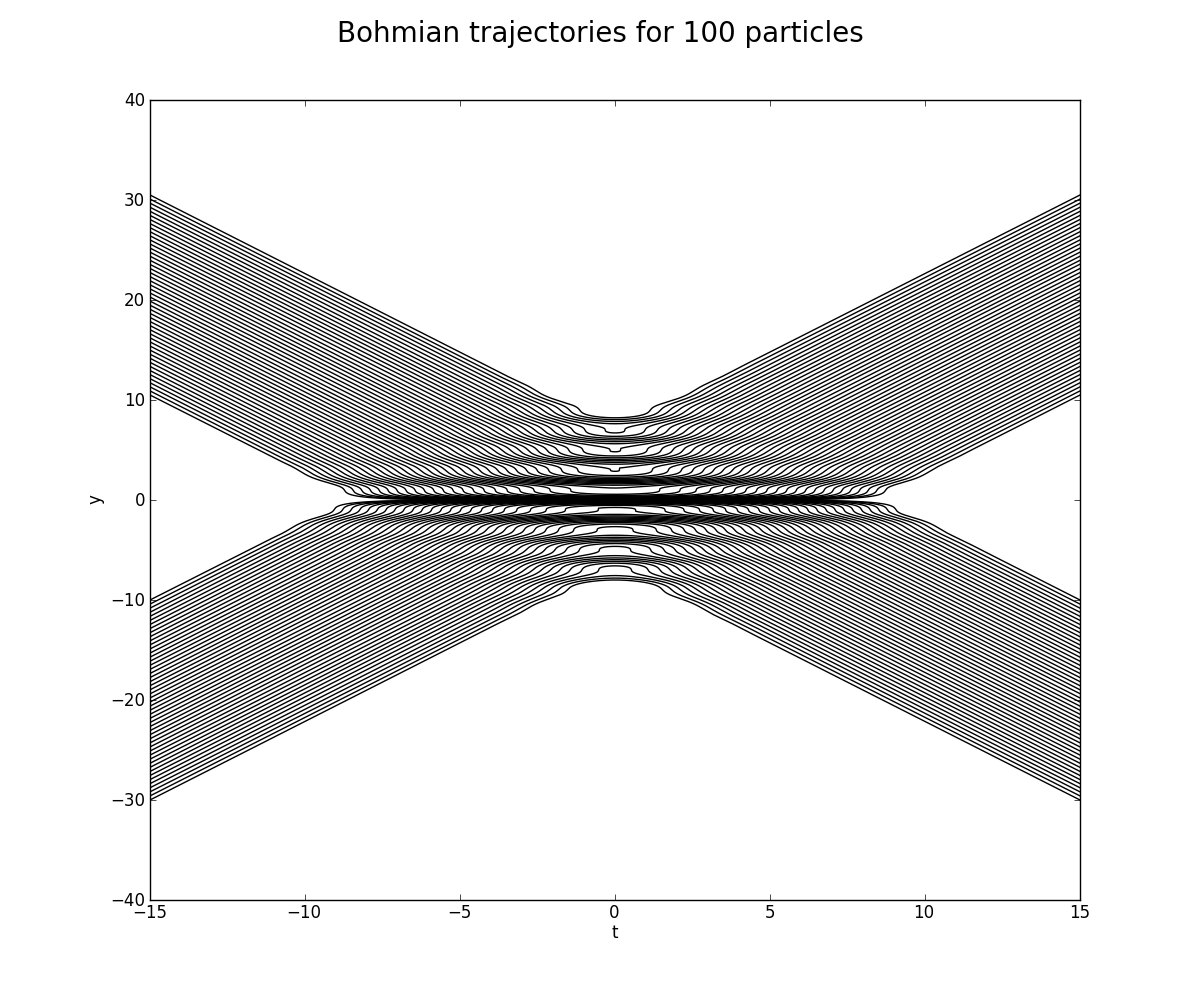
\includegraphics[scale=.5]{./imgs/100-bohmian-trajectories-b06f0d2cb50ffe27.png} \\}
    \caption{
      Bohmian trajectories plotted for wave function $\Psi$ describing two interfering Gaussian wave packets.
      100 particles are initially distributed with equidistant spacing on the $t=-15s$ axis.
      The bottom and top packets are offset by a 1/2 step to prevent symmetry over the $y=0$ axis.
    }
    \label{fig:interfering-trajectories}
  \end{figure}

  An instinctive interpretation of the interfering wave packets depicted in Figure \ref{fig:interfering} can lead one to assume that the two wave packets 
    head towards each other, interfere with each other, and then continue along their original path.
  The Bohmian trajectories show that as the wave packets $\psi_A$ and $\psi_B$ begin to interfere with one another the Bohmian trajectories begin detouring.
  When the wave packets are fully superimposed at $t=0s$, the trajectories are almost parallel with the $t$ axis, never crossing the $y=0$ axis. 
  As $\psi_A$ and $\psi_B$ continue propagating forward, the trajectories eventually turn around and head back towards the upper or lower region they originated from;
    creating another symmetry along the $t=0$ axis.
  This may indicate that the wave packets behave similarly and simply appear to continue along their original path.
  The familiar characteristics of Bohmian trajectories are still observed: the trajectories do not cross and veer from classical trajectories.
  Furthermore, the particle trajectories follow the pattern illustrated in Figure \ref{fig:interfering-trajectories} regardless of the initial distribution.

\section{Conclusion}

  In conclusion, Bohmian trajectories were numerically calculated with Python 2.7.2.
  A fourth-order Runge-Kutta was implemented to numerically solve the differential equation (\ref{eq:trajectories}) that describes the trajectories.
  Basic corroboration with known results was found and the expected interference patterns were observed.
  The effects of the quantum potential were noticeable as well via the deviations in the trajectories from their classical counterparts.
  All the Python scripts are referenced in the appendix and have the NumPy, SymPy and Matplotlib packages as dependencies.
  Computation times were relatively quick and given the open-sourced foundation of Python and its scientific packages the results can be freely replicated.

\pagebreak

\bibliographystyle{plain}
\bibliography{sources}

\pagebreak

\appendix
\newgeometry{left=2cm,right=2cm}

\section{Real and imaginary parts of the wave function for the double slit system}
\label{appendix:real-imag}
\verbatiminput{scripts/real-imaginary-graphs.py}
\pagebreak

\section{Imaginary surface over time of the wave function for a double slit system}
\label{appendix:imaginary-surface}
\verbatiminput{scripts/imaginary-surface.py}
\pagebreak 

\section{Bohmian trajectories for the double-slit setup}
\label{appendix:bohmian-trajectories}
\verbatiminput{scripts/bohm.py}
\pagebreak 

\section{Contour plot}
\label{appendix:contour-plot}
\verbatiminput{scripts/second-contour.py}
\pagebreak 

\section{Animated contour plot}
\label{appendix:contour-plot-animated}
\verbatiminput{scripts/second-contour-animated.py}
\pagebreak 

\section{Bohmian trajectories for the second setup}
\label{appendix:secondary-trajectories}
\verbatiminput{scripts/second.py}
\pagebreak 


\end{document}
